\subsubsection{Lookup table decoding}
A lookup table decoder works by generating the 
syndromes for the entire set of possible input errors, thus creating a 
table holding possible errors responsible for each possible syndrome.
The decoding then consists of merely assuming the minimum weight
error that leads to the known syndrome, since given low physical 
error rate, the least amount of errors leading to an error is the most
probable event.

This decoding scheme is particularly useful for small codes, as well 
as non-topological (random) LDPC (Low-Density-Parity-Check) codes, since
these cannot be decoded using graph theory.
A big issue with this decoding scheme is that generating lookup tables is
extremely computationally expensive ($O(2^n)$, since a syndrome must be computed
and stored for every possible error vector, having length n and 2 possibilities per
entry). 

This renders it practically
unfeasible to generate lookup tables for codes with a larger number
of total data qubits.

\begin{figure}[h!]
	\begin{center}
	\captionsetup{justification=centering,margin=2cm}
	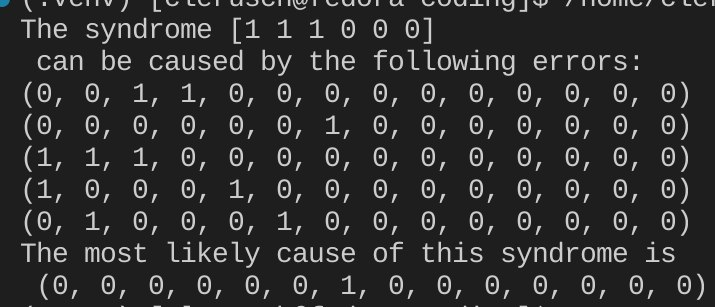
\includegraphics[scale=0.5]{./img/figures/X7errorlookup.png}\\
	\caption{Lookup table for an X error on the central qubit of
    a Steane code (qubit 7), generating code can be found in Appendix
    \ref{App: lookup_table}}
        
	\label{fig: lookup_table}
	\end{center}
\end{figure}

In Figure \ref{fig: lookup_table} is an example of the lookup table result for
an X error on qubit 7 (the central qubit) on the Steane code. 
The resulting syndrome is (1,1,1,0,0,0), with the first three
bits indicating the steane code faces X checks, and the second three bits
indicating the Steane code faces Z checks. 
The lookup table will return a set of many possible errors resulting in 
that syndrome, but simply choosing the one with the least number of errors 
(minimum weight) gives the correct error prediction.